\chapter{Esercizi}

\section{Esercizio da 3 punti}
Qui sono raccolti gli esercizi da tre punti dati fino ad ora, sono abbastanza standard e spesso vengono ripetuti.

\subsection{Abstract Factory}

Si disegni il diagramma delle classi che modella le componenti e le relazioni che intercorrono tra di esse all'interno del design pattern Abstract Factory (GoF). Si ponga particolare attenzione alle operazioni definite all'interno di ogni classe.

Si fornisca il diagramma delle classi del design pattern Abstract Factory, supponendo di avere due differenti tipologie di classi "prodotto", ProductA e ProductB, e due differenti loro concretizzazioni. Si individui inoltre nel diagramma come il design pattern Singleton possa essere utilizzato in concomitanza al pattern Abstract Factory.

\subsection{Adapter}

Riportare i diagrammi delle classi che caratterizzano le varianti del pattern Adapter, ossia Class Adapter e Object Adapter
e completare le seguenti affermazioni inserendo la corretta variante del pattern negli appositi spazi.
\begin{itemize}
\item Il pattern ... permette di adattare più tipi (Adaptee e le sue sottoclassi)
\item Il pattern ... permette di modificare alcune caratteristiche dell’Adaptee.
\end{itemize}

\begin{figure}
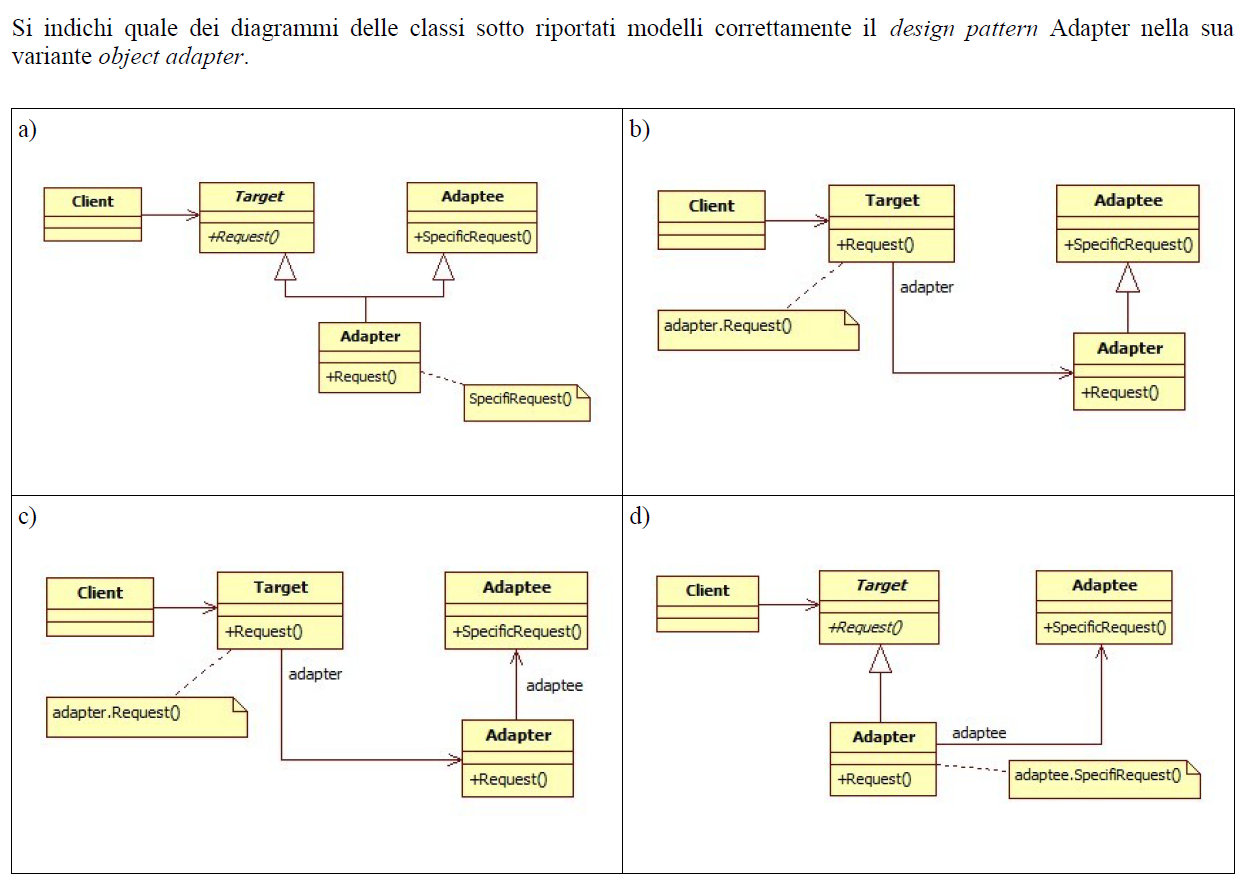
\includegraphics[width=1\textwidth]{res/img/Esercizi/es-adapter}
\end{figure}

\subsection{Builder}
\begin{figure}
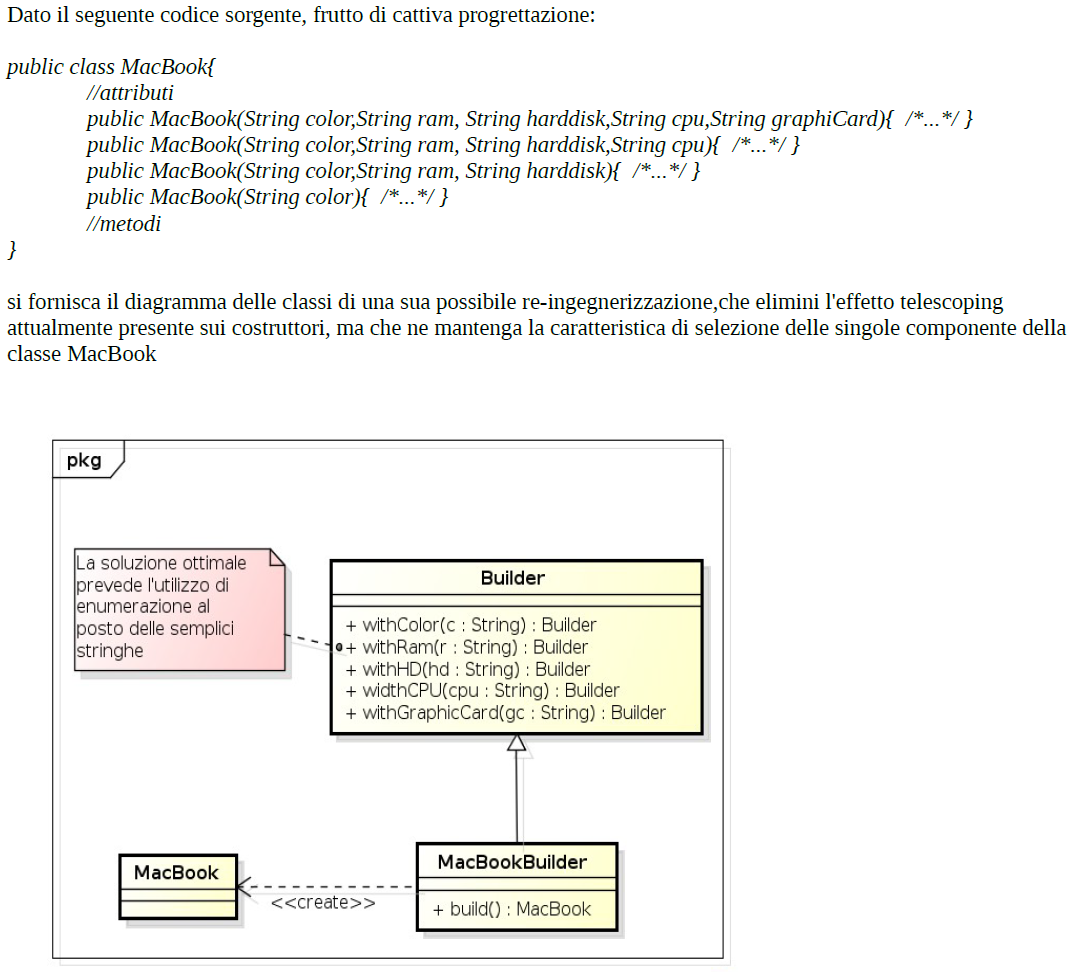
\includegraphics[width=1\textwidth]{res/img/Esercizi/es-builder}
\end{figure}

\subsection{Decorator}

Si disegni il diagramma delle classi che modella le componenti e le relazioni che intercorrono tra di esse all'interno del design pattern Decorator.

\subsection{Proxy}

Si disegni un diagramma delle classi che rappresenti il design pattern Proxy e se ne descriva brevemente un esempio
d'uso concreto.

\subsection{Observer}

I tipi astratti e concreti che partecipano al design pattern Observer sono almeno 4: Subject, Observer, ConcreteSubject e ConcreteObserver. Supponendo che esistano due osservatori concreti per un soggetto, aConcreteObserver e anotherConcreteObserver, si disegni il diagramma di sequenza che descrive le azioni conseguenti all'invocazione del metodo setState() sul soggetto, da parte di uno dei due osservatori.

\begin{figure}
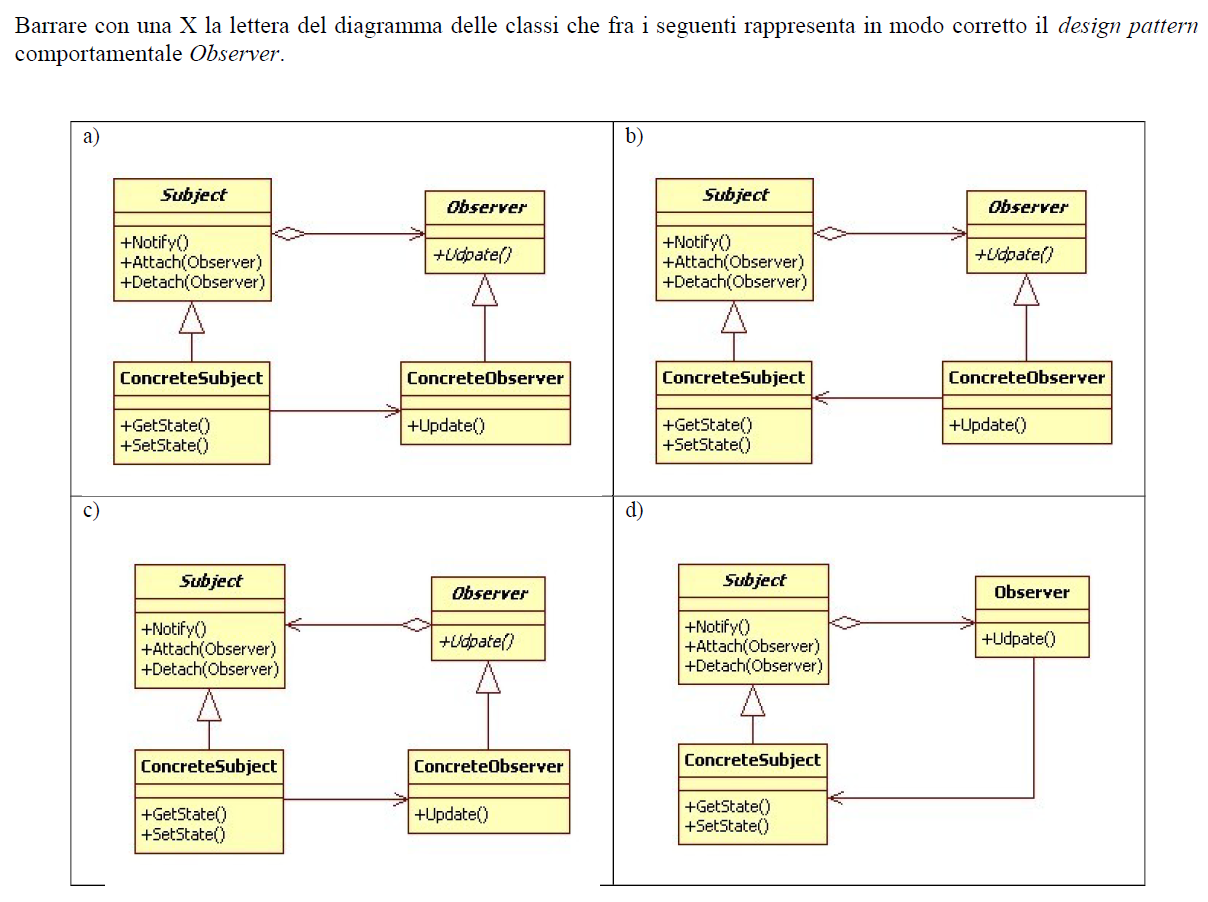
\includegraphics[width=1\textwidth]{res/img/Esercizi/es-observer}
\end{figure}

\begin{figure}
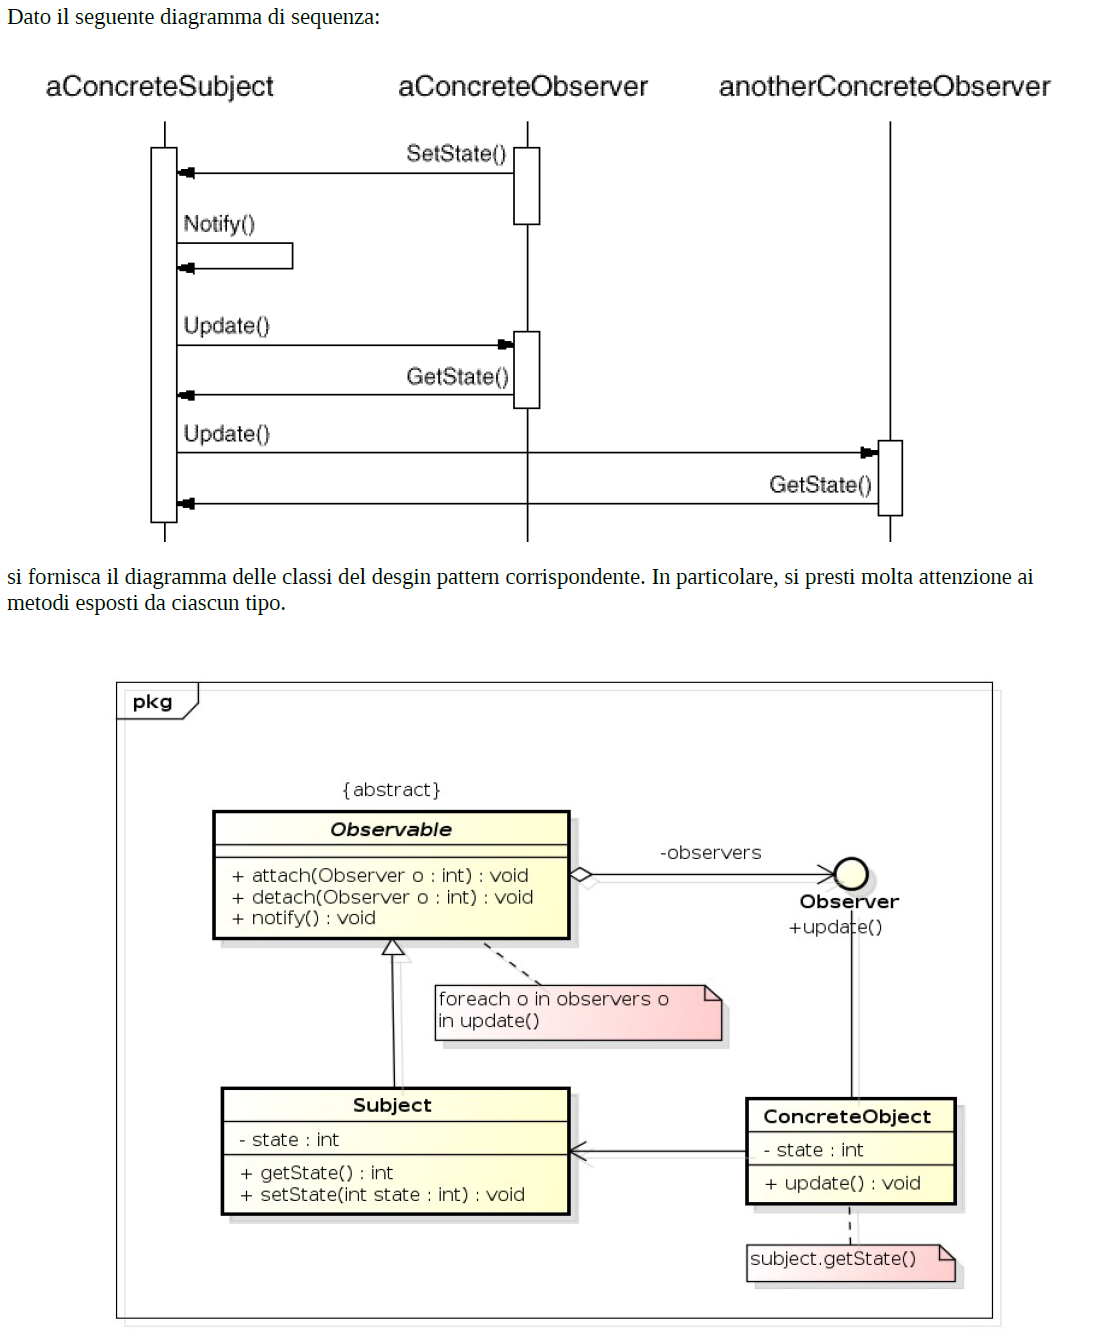
\includegraphics[width=1\textwidth]{res/img/Esercizi/es-observer2}
\end{figure}

\subsection{Diagrammi attività}
Per poter prendere un volo da Venezia per New York è necessario effettuare il check-in 1 (una) ora prima della partenza
del volo. Una viaggiatore residente a Padova decide di iniziare a fare le valigie 2 (due) ore prima dell'orario di partenza del
volo. Per arrivare all'aeroporto, quel viaggiatore decide di servirsi di un taxi e lo chiama nel momento in cui inizia a fare
le valigie. Se il taxi arrivasse prima che che il viaggiatore abbia terminato la preparazione delle valigie, il taxi dovrà
attendere (a tariffa). In caso contrario, terminando la preparazione delle valigie prima dell'arrivo del taxi, sarà il
v i a g g i a t o r e ad attendere.
Si disegni un diagramma di attività che modelli lo scenario descritto nel testo.
 
Una coppia di fidanzati decide di trascorrere il sabato sera in discoteca. Due ore prima dell'ora di uscita concordata, lei
inizia a prepararsi, il ragazzo però non si presenterà prima di mezz'ora dall'ora dell'appuntamento. Naturalmente, una
volta arrivato, il ragazzo dovrà pazientemente aspettare la fidanzata qualora essa non abbia ancora terminato di prepararsi.
Si disegni un diagramma di attività che modelli lo scenario descritto nel testo.

\begin{figure}
\includegraphics[width=0.8\textwidth]{res/img/Esercizi/es-diagrammaAttività1}
\end{figure}

\begin{figure}
\includegraphics[width=0.8\textwidth]{res/img/Esercizi/es-diagrammaAttività2}
\end{figure}

\subsection{MVC}

\begin{figure}
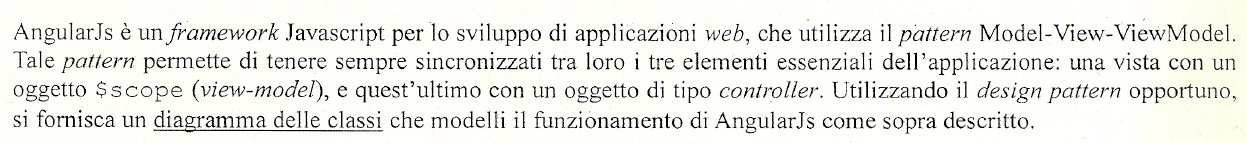
\includegraphics[width=0.8\textwidth]{res/img/Esercizi/es-angular}
\end{figure}

\begin{figure}
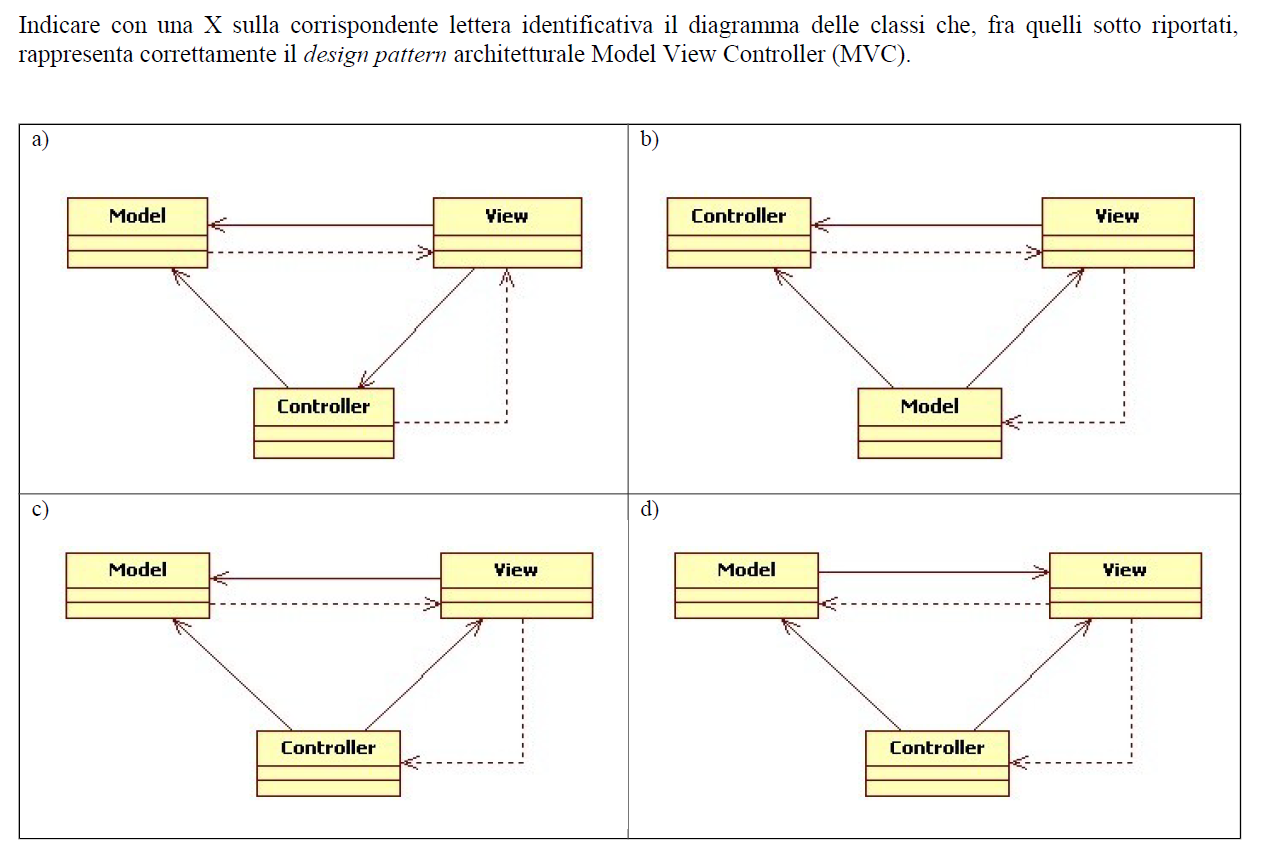
\includegraphics[width=1\textwidth]{res/img/Esercizi/es-mvc}
\end{figure}

\subsection{Altro}
\begin{figure}
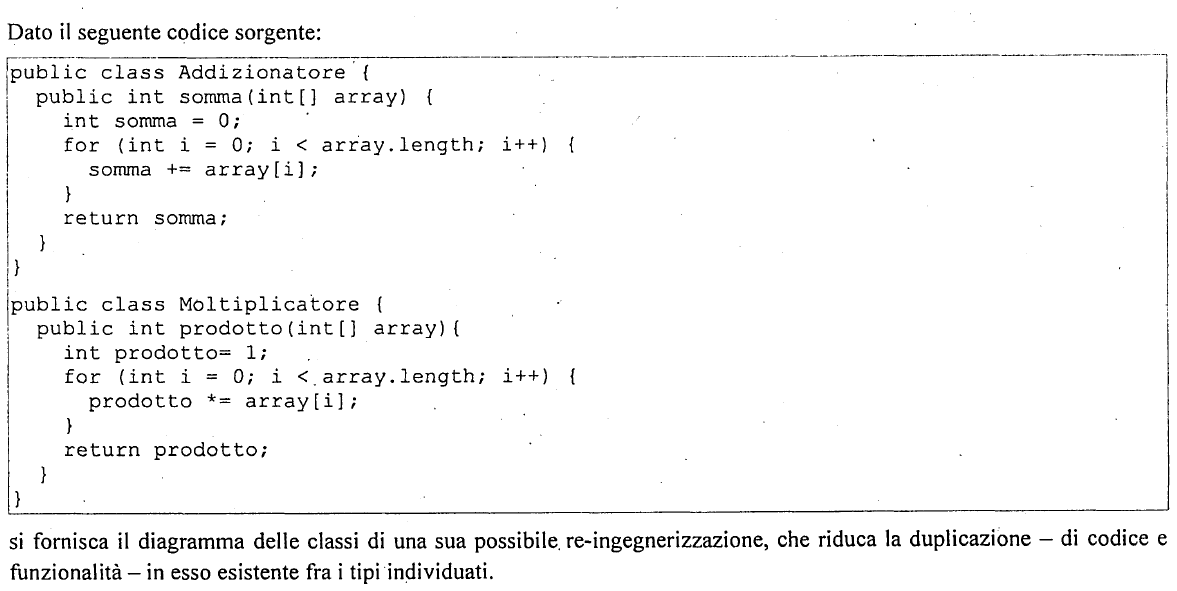
\includegraphics[width=1\textwidth]{res/img/Esercizi/es-codice}
\end{figure}
